%% bare_conf.tex
%% V1.4b
%% 2015/08/26
%% by Michael Shell
%% See:
%% http://www.michaelshell.org/
%% for current contact information.
%%
%% This is a skeleton file demonstrating the use of IEEEtran.cls
%% (requires IEEEtran.cls version 1.8b or later) with an IEEE
%% conference paper.
%%
%% Support sites:
%% http://www.michaelshell.org/tex/ieeetran/
%% http://www.ctan.org/pkg/ieeetran
%% and
%% http://www.ieee.org/

%%*************************************************************************
%% Legal Notice:
%% This code is offered as-is without any warranty either expressed or
%% implied; without even the implied warranty of MERCHANTABILITY or
%% FITNESS FOR A PARTICULAR PURPOSE!
%% User assumes all risk.
%% In no event shall the IEEE or any contributor to this code be liable for
%% any damages or losses, including, but not limited to, incidental,
%% consequential, or any other damages, resulting from the use or misuse
%% of any information contained here.
%%
%% All comments are the opinions of their respective authors and are not
%% necessarily endorsed by the IEEE.
%%
%% This work is distributed under the LaTeX Project Public License (LPPL)
%% ( http://www.latex-project.org/ ) version 1.3, and may be freely used,
%% distributed and modified. A copy of the LPPL, version 1.3, is included
%% in the base LaTeX documentation of all distributions of LaTeX released
%% 2003/12/01 or later.
%% Retain all contribution notices and credits.
%% ** Modified files should be clearly indicated as such, including  **
%% ** renaming them and changing author support contact information. **
%%*************************************************************************


% *** Authors should verify (and, if needed, correct) their LaTeX system  ***
% *** with the testflow diagnostic prior to trusting their LaTeX platform ***
% *** with production work. The IEEE's font choices and paper sizes can   ***
% *** trigger bugs that do not appear when using other class files.       ***                          ***
% The testflow support page is at:
% http://www.michaelshell.org/tex/testflow/



\documentclass[conference]{IEEEtran}
% Some Computer Society conferences also require the compsoc mode option,
% but others use the standard conference format.
%
% If IEEEtran.cls has not been installed into the LaTeX system files,
% manually specify the path to it like:
% \documentclass[conference]{../sty/IEEEtran}





% Some very useful LaTeX packages include:
% (uncomment the ones you want to load)


% *** MISC UTILITY PACKAGES ***
%
%\usepackage{ifpdf}
% Heiko Oberdiek's ifpdf.sty is very useful if you need conditional
% compilation based on whether the output is pdf or dvi.
% usage:
% \ifpdf
%   % pdf code
% \else
%   % dvi code
% \fi
% The latest version of ifpdf.sty can be obtained from:
% http://www.ctan.org/pkg/ifpdf
% Also, note that IEEEtran.cls V1.7 and later provides a builtin
% \ifCLASSINFOpdf conditional that works the same way.
% When switching from latex to pdflatex and vice-versa, the compiler may
% have to be run twice to clear warning/error messages.






% *** CITATION PACKAGES ***
%
%\usepackage{cite}
% cite.sty was written by Donald Arseneau
% V1.6 and later of IEEEtran pre-defines the format of the cite.sty package
% \cite{} output to follow that of the IEEE. Loading the cite package will
% result in citation numbers being automatically sorted and properly
% "compressed/ranged". e.g., [1], [9], [2], [7], [5], [6] without using
% cite.sty will become [1], [2], [5]--[7], [9] using cite.sty. cite.sty's
% \cite will automatically add leading space, if needed. Use cite.sty's
% noadjust option (cite.sty V3.8 and later) if you want to turn this off
% such as if a citation ever needs to be enclosed in parenthesis.
% cite.sty is already installed on most LaTeX systems. Be sure and use
% version 5.0 (2009-03-20) and later if using hyperref.sty.
% The latest version can be obtained at:
% http://www.ctan.org/pkg/cite
% The documentation is contained in the cite.sty file itself.






% *** GRAPHICS RELATED PACKAGES ***
%
\ifCLASSINFOpdf
  % \usepackage[pdftex]{graphicx}
  % declare the path(s) where your graphic files are
  % \graphicspath{{../pdf/}{../jpeg/}}
  % and their extensions so you won't have to specify these with
  % every instance of \includegraphics
  % \DeclareGraphicsExtensions{.pdf,.jpeg,.png}
\else
  % or other class option (dvipsone, dvipdf, if not using dvips). graphicx
  % will default to the driver specified in the system graphics.cfg if no
  % driver is specified.
  % \usepackage[dvips]{graphicx}
  % declare the path(s) where your graphic files are
  % \graphicspath{{../eps/}}
  % and their extensions so you won't have to specify these with
  % every instance of \includegraphics
  % \DeclareGraphicsExtensions{.eps}
\fi
% graphicx was written by David Carlisle and Sebastian Rahtz. It is
% required if you want graphics, photos, etc. graphicx.sty is already
% installed on most LaTeX systems. The latest version and documentation
% can be obtained at:
% http://www.ctan.org/pkg/graphicx
% Another good source of documentation is "Using Imported Graphics in
% LaTeX2e" by Keith Reckdahl which can be found at:
% http://www.ctan.org/pkg/epslatex
%
% latex, and pdflatex in dvi mode, support graphics in encapsulated
% postscript (.eps) format. pdflatex in pdf mode supports graphics
% in .pdf, .jpeg, .png and .mps (metapost) formats. Users should ensure
% that all non-photo figures use a vector format (.eps, .pdf, .mps) and
% not a bitmapped formats (.jpeg, .png). The IEEE frowns on bitmapped formats
% which can result in "jaggedy"/blurry rendering of lines and letters as
% well as large increases in file sizes.
%
% You can find documentation about the pdfTeX application at:
% http://www.tug.org/applications/pdftex





% *** MATH PACKAGES ***
%
%\usepackage{amsmath}
% A popular package from the American Mathematical Society that provides
% many useful and powerful commands for dealing with mathematics.
%
% Note that the amsmath package sets \interdisplaylinepenalty to 10000
% thus preventing page breaks from occurring within multiline equations. Use:
%\interdisplaylinepenalty=2500
% after loading amsmath to restore such page breaks as IEEEtran.cls normally
% does. amsmath.sty is already installed on most LaTeX systems. The latest
% version and documentation can be obtained at:
% http://www.ctan.org/pkg/amsmath





% *** SPECIALIZED LIST PACKAGES ***
%
%\usepackage{algorithmic}
% algorithmic.sty was written by Peter Williams and Rogerio Brito.
% This package provides an algorithmic environment fo describing algorithms.
% You can use the algorithmic environment in-text or within a figure
% environment to provide for a floating algorithm. Do NOT use the algorithm
% floating environment provided by algorithm.sty (by the same authors) or
% algorithm2e.sty (by Christophe Fiorio) as the IEEE does not use dedicated
% algorithm float types and packages that provide these will not provide
% correct IEEE style captions. The latest version and documentation of
% algorithmic.sty can be obtained at:
% http://www.ctan.org/pkg/algorithms
% Also of interest may be the (relatively newer and more customizable)
% algorithmicx.sty package by Szasz Janos:
% http://www.ctan.org/pkg/algorithmicx




% *** ALIGNMENT PACKAGES ***
%
%\usepackage{array}
% Frank Mittelbach's and David Carlisle's array.sty patches and improves
% the standard LaTeX2e array and tabular environments to provide better
% appearance and additional user controls. As the default LaTeX2e table
% generation code is lacking to the point of almost being broken with
% respect to the quality of the end results, all users are strongly
% advised to use an enhanced (at the very least that provided by array.sty)
% set of table tools. array.sty is already installed on most systems. The
% latest version and documentation can be obtained at:
% http://www.ctan.org/pkg/array


% IEEEtran contains the IEEEeqnarray family of commands that can be used to
% generate multiline equations as well as matrices, tables, etc., of high
% quality.




% *** SUBFIGURE PACKAGES ***
%\ifCLASSOPTIONcompsoc
%  \usepackage[caption=false,font=normalsize,labelfont=sf,textfont=sf]{subfig}
%\else
%  \usepackage[caption=false,font=footnotesize]{subfig}
%\fi
% subfig.sty, written by Steven Douglas Cochran, is the modern replacement
% for subfigure.sty, the latter of which is no longer maintained and is
% incompatible with some LaTeX packages including fixltx2e. However,
% subfig.sty requires and automatically loads Axel Sommerfeldt's caption.sty
% which will override IEEEtran.cls' handling of captions and this will result
% in non-IEEE style figure/table captions. To prevent this problem, be sure
% and invoke subfig.sty's "caption=false" package option (available since
% subfig.sty version 1.3, 2005/06/28) as this is will preserve IEEEtran.cls
% handling of captions.
% Note that the Computer Society format requires a larger sans serif font
% than the serif footnote size font used in traditional IEEE formatting
% and thus the need to invoke different subfig.sty package options depending
% on whether compsoc mode has been enabled.
%
% The latest version and documentation of subfig.sty can be obtained at:
% http://www.ctan.org/pkg/subfig




% *** FLOAT PACKAGES ***
%
%\usepackage{fixltx2e}
% fixltx2e, the successor to the earlier fix2col.sty, was written by
% Frank Mittelbach and David Carlisle. This package corrects a few problems
% in the LaTeX2e kernel, the most notable of which is that in current
% LaTeX2e releases, the ordering of single and double column floats is not
% guaranteed to be preserved. Thus, an unpatched LaTeX2e can allow a
% single column figure to be placed prior to an earlier double column
% figure.
% Be aware that LaTeX2e kernels dated 2015 and later have fixltx2e.sty's
% corrections already built into the system in which case a warning will
% be issued if an attempt is made to load fixltx2e.sty as it is no longer
% needed.
% The latest version and documentation can be found at:
% http://www.ctan.org/pkg/fixltx2e


%\usepackage{stfloats}
% stfloats.sty was written by Sigitas Tolusis. This package gives LaTeX2e
% the ability to do double column floats at the bottom of the page as well
% as the top. (e.g., "\begin{figure*}[!b]" is not normally possible in
% LaTeX2e). It also provides a command:
%\fnbelowfloat
% to enable the placement of footnotes below bottom floats (the standard
% LaTeX2e kernel puts them above bottom floats). This is an invasive package
% which rewrites many portions of the LaTeX2e float routines. It may not work
% with other packages that modify the LaTeX2e float routines. The latest
% version and documentation can be obtained at:
% http://www.ctan.org/pkg/stfloats
% Do not use the stfloats baselinefloat ability as the IEEE does not allow
% \baselineskip to stretch. Authors submitting work to the IEEE should note
% that the IEEE rarely uses double column equations and that authors should try
% to avoid such use. Do not be tempted to use the cuted.sty or midfloat.sty
% packages (also by Sigitas Tolusis) as the IEEE does not format its papers in
% such ways.
% Do not attempt to use stfloats with fixltx2e as they are incompatible.
% Instead, use Morten Hogholm'a dblfloatfix which combines the features
% of both fixltx2e and stfloats:
%
% \usepackage{dblfloatfix}
% The latest version can be found at:
% http://www.ctan.org/pkg/dblfloatfix




% *** PDF, URL AND HYPERLINK PACKAGES ***
%
%\usepackage{url}
% url.sty was written by Donald Arseneau. It provides better support for
% handling and breaking URLs. url.sty is already installed on most LaTeX
% systems. The latest version and documentation can be obtained at:
% http://www.ctan.org/pkg/url
% Basically, \url{my_url_here}.




% *** Do not adjust lengths that control margins, column widths, etc. ***
% *** Do not use packages that alter fonts (such as pslatex).         ***
% There should be no need to do such things with IEEEtran.cls V1.6 and later.
% (Unless specifically asked to do so by the journal or conference you plan
% to submit to, of course. )


% correct bad hyphenation here
\hyphenation{op-tical net-works semi-conduc-tor}
\usepackage{graphicx}
\usepackage{amssymb}
\usepackage{subfigure}
\usepackage{xspace}
\usepackage[british,UKenglish,USenglish,english,american]{babel}


\newcommand{\tabincell}[2]{\begin{tabular}{@{}#1@{}}#2\end{tabular}}
\newcommand{\DSVMP}{\textsc{Dsvmp}\xspace}

\IEEEoverridecommandlockouts

\renewcommand{\thefootnote}{\fnsymbol{footnote}}

%\def\@IEEEsectpunct{.\ \,}
%\def\paragraph{\@startsection{paragraph}{4}{\z@}{1.5ex plus 1.5ex minus 0.5ex}%
%{0ex}{\normalfont\normalsize\sffamily\bfseries}}
\makeatother

\begin{document}

%
\title{Exploiting Dynamic Instruction Scheduling for VM-Based Code Obfuscation}


\author{\IEEEauthorblockN{Kaiyuan Kuang\IEEEauthorrefmark{2}, Zhanyong Tang\IEEEauthorrefmark{2}\IEEEauthorrefmark{1}\thanks{*Corresponding author. Email address: zytang@nwu.edu.cn}, Xiaoqing Gong\IEEEauthorrefmark{2}, Dingyi Fang\IEEEauthorrefmark{2}, Xiaojiang Chen\IEEEauthorrefmark{2},\\
Tianzhang Xing\IEEEauthorrefmark{2}, Guixin Ye\IEEEauthorrefmark{2}, Jie Zhang\IEEEauthorrefmark{2}, Zheng Wang\IEEEauthorrefmark{3}}
\IEEEauthorblockA{\IEEEauthorrefmark{2}School of Information Science and Technology, Northwest University, Xi'an, 710127, P.R. China.\\
\IEEEauthorrefmark{3}School of Computing and Communications, Lancaster University, UK\\
%\IEEEauthorrefmark{2}\{xx, zytang, xiaoqinggong, dyf, ...\}@nwu.edu.cn, \IEEEauthorrefmark{3}z.wang@lancaster.ac.uk
}
%NWU-Irdeto IoT-Information Security Joint Laboratory\\
%$^*$Correspondence should be addressed to Zhanyong Tang, Email: zytang@nwu.edu.cn}
}
%\and
%\IEEEauthorblockN{Homer Simpson}
%\IEEEauthorblockA{Twentieth Century Fox\\
%Springfield, USA\\
%Email: homer@thesimpsons.com}
%\and
%\IEEEauthorblockN{James Kirk\\ and Montgomery Scott}
%\IEEEauthorblockA{Starfleet Academy\\
%San Francisco, California 96678--2391\\
%Telephone: (800) 555--1212\\
%Fax: (888) 555--1212}

% conference papers do not typically use \thanks and this command
% is locked out in conference mode. If really needed, such as for
% the acknowledgment of grants, issue a \IEEEoverridecommandlockouts
% after \documentclass

% for over three affiliations, or if they all won't fit within the width
% of the page, use this alternative format:
%
%\author{\IEEEauthorblockN{Michael Shell\IEEEauthorrefmark{1},
%Homer Simpson\IEEEauthorrefmark{2},
%James Kirk\IEEEauthorrefmark{3},
%Montgomery Scott\IEEEauthorrefmark{3} and
%Eldon Tyrell\IEEEauthorrefmark{4}}
%\IEEEauthorblockA{\IEEEauthorrefmark{1}School of Electrical and Computer Engineering\\
%Georgia Institute of Technology,
%Atlanta, Georgia 30332--0250\\ Email: see http://www.michaelshell.org/contact.html}
%\IEEEauthorblockA{\IEEEauthorrefmark{2}Twentieth Century Fox, Springfield, USA\\
%Email: homer@thesimpsons.com}
%\IEEEauthorblockA{\IEEEauthorrefmark{3}Starfleet Academy, San Francisco, California 96678-2391\\
%Telephone: (800) 555--1212, Fax: (888) 555--1212}
%\IEEEauthorblockA{\IEEEauthorrefmark{4}Tyrell Inc., 123 Replicant Street, Los Angeles, California 90210--4321}}




% use for special paper notices
%\IEEEspecialpapernotice{(Invited Paper)}




% make the title area
\maketitle

% As a general rule, do not put math, special symbols or citations
% in the abstract
\begin{abstract}
\par Code virtualization building upon virtual machine (VM) technologies is
emerging as a viable method for implementing code obfuscation to protect
programs against unauthorized analysis. State-of-the-art VM-based
protection approaches use a fixed scheduling structure where the
program follows a single, static execution path for the same input. Such
approaches, however, are vulnerable to dynamic cumulative attacks where the
attacker can reuse knowledge extracted from previously seen software
to crack applications using similar protection schemes. This paper
presents \DSVMP, a novel VM-based code obfuscation approach for protecting software
against dynamic cumulative attacks.
\DSVMP brings together two techniques to provide stronger
code protection than prior VM-based schemes.
Firstly, it uses a dynamic instruction
scheduler to randomly direct the program to execute different paths without
violating the correctness across different runs. By randomly choosing
the program execution paths, the application exposes diverse behavior, making
it much more difficult for an attacker to reuse the knowledge collected from
previous runs or similar applications to perform attacks. Secondly, it employs
multiple VMs to further obfuscate the relationship between VM bytecode and
their interpreters, making code analysis even harder. We have implemented
\DSVMP  in a prototype system and evaluated it using a set of widely used applications.
Experimental results show that \DSVMP provides stronger protection with lower runtime overhead
and code size when compared to two commercial VM-based code obfuscation tools.
\end{abstract}

\begin{IEEEkeywords}
Code virtualization; Code Obfuscation; Dynamic cumulative attack
\end{IEEEkeywords}
% no keywords




% For peer review papers, you can put extra information on the cover
% page as needed:
% \ifCLASSOPTIONpeerreview
% \begin{center} \bfseries EDICS Category: 3-BBND \end{center}
% \fi
%
% For peerreview papers, this IEEEtran command inserts a page break and
% creates the second title. It will be ignored for other modes.
\IEEEpeerreviewmaketitle



\section{Introduction}
Unauthorized code analysis and modification based on software reverse
engineering is a critical issue for software companies. Such attacks can lead to
a number of undesired outcomes, including cheating in games, unauthorized
used of software, pirated pay-tv etc. Industry is looking for techniques to
address this issue to prevent tampering and deter reverse engineering of software systems. By making the
sensitive parts of the program difficult to be tracked or analyzed, code obfuscation is a potential
solution for the problem.



Code virtualization building upon a virtual machine (VM) is emerging as a
promising way for implementing code
obfuscation~\cite{1Themida,2CV,3Vmprotect,5fang2011multi,6ming2011software,7wang2014tdvmp,8wang2013nislvmp}.
The idea of VM-based protection is to replace the native machine code with
virtual bytecodes which will then be translated into native machine code at runtime. Using a VM-based scheme, the execution path of the
obfuscated code is controlled by a virtual instruction scheduler.
A typical
scheduler consists of two parts: a dispatcher that determines which virtual
instruction (i.e. bytecode) is ready for execution, and an instruction handler that translates
the bytecode into native machine code to be executed on the underlying
hardware. This process replaces the original program instructions with
bespoke bytecodes, allowing developers to conceal the purpose or logic of sensitive code regions.


Prior work on VM-based software protection has primarily focused on making
a single set of bytecode more complicate and used only one virtual scheduler.
Such approaches rely on the assumption that the scheduler and the bytecode
instruction set are difficult to be analyzed in most practical runtime
environments. However, research has shown that is a rather unreliable
assumption~\cite{10falliere2009inside} under \emph{dynamic cumulative attacks} where an adversary can easily
reuse  knowledge extracted from other
applications protected with the same set of VM tools to preform reverse engineering. 
To protect software against dynamic cumulative attacks, it is vital important to introduce a certain degree of uncertainty and diversity into program execution~\cite{4collberg}.

This paper presents \DSVMP, a novel VM-based code protection scheme to
address the problem of dynamic cumulative attacks.  Our key insight is that
it will be much more difficult for the attacker to analyze the code if the
program behaves differently in different runs. We achieve this by introducing
rich uncertainty into the program execution and bytecode interpretation. To do so, \DSVMP
exploits a flexible, multi-dispatched scheme for code scheduling and interpretation. Unlike prior work where a program always follows a
single, fixed execution path for the same input across different runs, the
\DSVMP scheduler directs the program to execute a randomly selected path when
executing a protected code region. As a result, the program follows different
execution paths in different runs and has non-deterministic behavior. Our carefully
designed scheme ensures that the program will produces a deterministic output
for the same input despite the execution paths might look differently from
the attacker's perspective. To analyze software protected under \DSVMP, the
adversary is forced to use a large number of trail runs to understand how the
program algorithm works. As a result, this significantly increases the cost for code reverse-engineering.


%Uncertainty and diversity are keys for deterring dynamic cumulative attacks.
In addition to dynamic instruction scheduling, \DSVMP brings together two other techniques to increase diversity of program behaviour.
Firstly, \DSVMP provides
 multiple handlers, which are implemented using different algorithms and data structures, to translate a bytecode instruction to native code.
Handlers for a particular bytecode
all generate an identical output for the same input, but their execution paths and data accessing patterns are different from each other.
During runtime,  our VM instruction scheduler
randomly selects an bytecode handler to translate a virtual instruction to the native machine code.
Since the
choice of handlers is randomly determined at runtime for each bytecode
instruction and the implementation of different handlers are different, the dynamic program execution path is likely to be different in
different runs. Secondly, \DSVMP employs a multi-VM scheme so that various
code regions can be protected using different bytecode instruction sets and VM
implementations. This further increases diversity of the program,
making it even harder for an adversary to analyze
the software behavior or reuse knowledge extracted from other software
products (as different products are likely to be protected by different
bytecodes instructions and VM implementations). 


The whole is greater than the sum of the parts.
These techniques, putting together, enable \DSVMP to provide stronger code protection than any of the VM-based techniques seen so far. 
We have evaluated \DSVMP on four widely used hashing and encryption applications:  \texttt{md5},
\texttt{aescrypt}, \texttt{bcrypt}, and \texttt{gzip}. Experimental results show that \DSVMP provides stronger protection
with lower runtime overhead and smaller code size compared to two commercial VM-based code obfuscation tools: Code Virtualizer~\cite{2CV} and VMProtect~\cite{3Vmprotect}.


This paper makes the following contributions:
\begin{itemize}
  \item It presents a dynamic scheduling structure for VM-based code obfuscation to protect software against dynamic cumulative attacks.
  \item It is the first to apply multiple VMs to enhance diversity of code obfuscation.
  \item It demonstrates that the proposed scheme is effective in protecting real-world software applications.
\end{itemize}


%\par The rest of this paper is organized as follows. Section II introduces the working principle of classical VM-based code obfuscation techniques. Section III describes the attacking scenario. Section IV gives an overview of \DSVMP, which is followed by a detailed description of the design in Section V. Section VI uses a case study to demonstrate protection scheme provided by \DSVMP. Evaluation results are presented in Sections VII and VIII before we discuss the related work in Section IX. Finally, Section X concludes the paper.



\section{Background}
VM-based code obfuscation transform native instructions of the protected code regions to virtual instructions. The virtual instructions are encoded into bytecode  which will be translated to native machine code at runtime using a set of bytecode handlers. Indeed, a new VM section is inserted to the end of target program and remaining code is kept intact, thus entry point of the protected code is redirected into VM section. In general, classic VM bytecode execution is stack based style, and need for a virtual context (VMcontext), which usually is a block of memory that contains the virtual registers and flags. The return value of each bytecode is saved in virtual registers, for next bytecode execution. When entering the VM, the native context is stored in the VMcontext to initialize the virtual context, and when exiting the VM, native context will be restored based on the virtual context. The VM interpreter is the core of the VM, which consists of a dispatcher and the handling procedures of bytecode instructions (handlers). The main loop that iterates through three phases for every instruction: decode, dispatch and execute\cite{9ghosh2012replacement}. Werewolf or assassin, dispatcher fetch a bytecode, then decode and dispatch a handler to interpret it. Obviously, the adversary can crack the original software easily if he understands the virtual interpreter and decodes mapping between two instruction sets (binary codes and bytecodes).


\textbf{Dynamic cumulative attack} Figure\ref{fig:Fig.1} illustrates how
an attacker can perform attack by reusing knowledge extracted from the
previous runs of the same application or other applications (that are
protected using the same VM scheme).In general, there is a positive
correlation that the more times the attack is, the more reusable attack
knowledge will be mastered, and eventually compromises the target
software. If a software shows dynamically variant execution paths in different run times, which can destroy this kind of positive correlation. Our work is to achieve this purpose.


\begin{figure}[t]%ͼ1
    \centering
    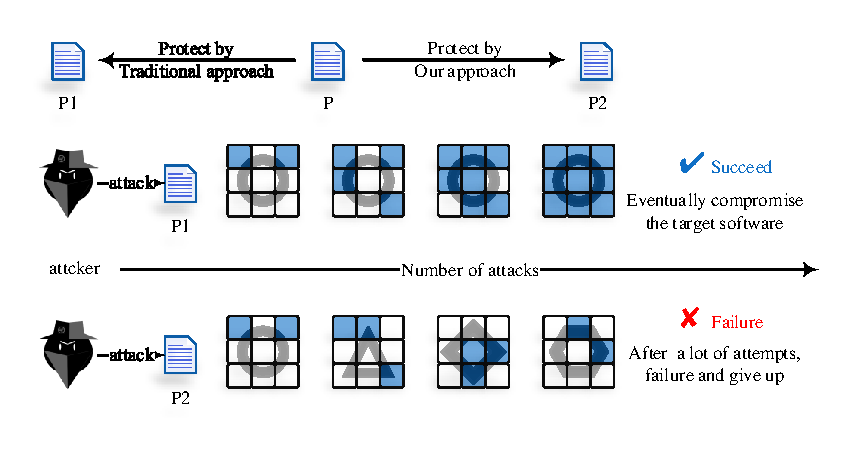
\includegraphics[width=1.0\columnwidth]{figure/figone.pdf}
    \caption{Diversity affects effectiveness of attack. Software crack like puzzle game, the dark small square represents the reusable attack knowledge. A single structure can be defeated by cumulative attack easily, but diversity of structure can against such attacks effectively.}\label{fig:Fig.1}
\end{figure}


\section{The Attack Model}
We assume that the adversary has an executable program of the target software, and he can run it in the malicious host environment\cite{11collberg2002watermarking}. The adversary has necessary attack technology, he can access memory or registers and trace instructions, and even can change the original instructions and control flows by using some static and dynamic analysis tools, like "IDA"\cite{14Idapro}, "Ollydbg"\cite{15Ollydbg}, "Sysinternals suite"\cite{16Sysinternalssuite}, etc. His goal is to completely reverse the internal implementation of target program, and then use that knowledge to grab benefits for his own.
\par The classical approach to reverse engineer a VM-protected program is consists of following steps\cite{10falliere2009inside,17rolles2009unpacking}. First, reverse engineer the virtual interpreter which consists of dispatcher and handling procedures, the attacker needs to locate them and analyzes what they do. Then, use this information to collect the individual bytecode instructions and its mapping relationship with the handling procedures. Finally, recover original internal logic implementation of the target program. Once an attacker has analyzed some information about the structure, he could reuse it for continually analyzing. The cumulative attack is the attacker accumulates these reusable attack knowledges through repeated reverse analysis, and eventually compromise the target software. In our attack model, the adversary is a skilled attacker, he can use any analysis tools and be familiar with the implementation mechanisms of VM, and he follows the steps described above while reverse engineering a VM-obfuscated program.

\section{\DSVMP Overview}
\DSVMP is a fine-grained code virtualized software protection system that can provide a resolution to make control flow in different ways every time.
\par Following the common practice in VM-based protection, \DSVMP also focus on protecting the critical code that has significant value, which can improve the performance. \DSVMP's infrastructure also includes the dispatcher to fetch the bytecode instructions. The implementation process of \DSVMP at a high level goes through the following steps, as shown in Figure\ref{fig:Fig.2}.
\par \textbf{Step1:} Locate the target code segment, and use the disassembling engine to get the x86 instructions.
\par \textbf{Step2:} Map x86 instructions to virtual instructions based on VIS (Virtual Instruction Set).
\par \textbf{Step3:} Different from the traditional VM, \DSVMP improved the handler and dispatcher that add the structural control unit for them, which are used to realize the uncertainty structure and multi-VM scheduling.
\par \textbf{Step4:} Generate multiple sets of handlers and dispatchers. We use the \emph{VMNum} ($>$=1) and \emph{DisNum} ($>$=1) to indicate the number of VM and dispatcher respectively. The original handlers set will be obfuscated \emph{VMNum} times by using the deformation engine, and disrupt the sequences of each set of handlers. Then we get \emph{VMNum} sets of equivalent but different forms of handlers. Similarly, generate \emph{DisNum} dispatchers which have the same function but, with various forms.
\par \textbf{Step5:} Generate \emph{2*VMNum} sets of driver-data. Map VI and handlers then generates \emph{VMNum} sets driver-data (which is composed of the handler's serial number and its parameters.). And the offset value (that between the current handler and next handler) creates the rest of \emph{VMNum} sets driver-data.
\par \textbf{Step6:} Construct the multiple VM, which is composed of the \emph{VMNum} sets of handlers and \emph{2*VMNum} sets of driver-data.
\par \textbf{Step7:} Insert a new section at the end of protected file, which contains \emph{VMNum} VMs and other VM components such as dispatcher, VMcontext, VMinit and VMexit etc.
%\par The next few sections elaborate on the above steps, providing the technical details.

\section{System Design For \DSVMP}
This paper introduces \DSVMP, which distribute a unique structure at every runtimes. We outlined a practical approach that provides tailor-made driver-data. The diversity of \DSVMP depends on two parts of the work: the diversified scheduling structure and the Multi-VM. In this section, we will present the details of our solution.
\begin{figure}[t]
  \centering
  % Requires \usepackage{graphicx}
  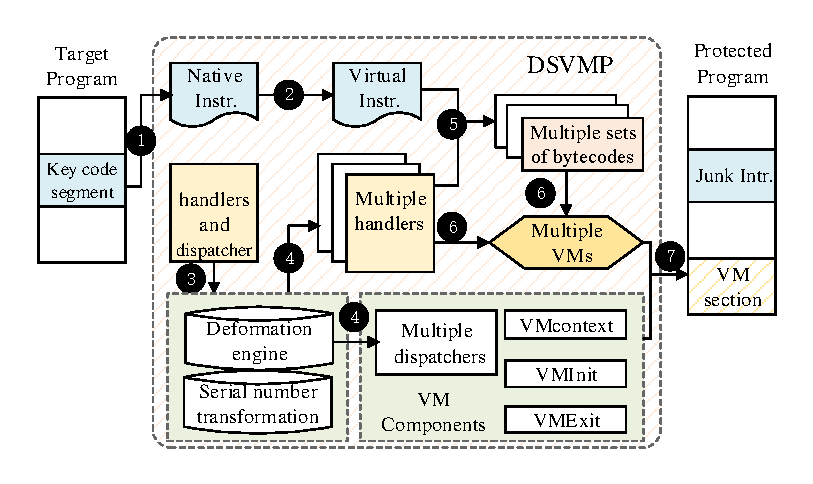
\includegraphics[width=1.0\columnwidth]{figure/figtwo.pdf}
  \caption{Overview of \DSVMP. First get the VI from critical codes, and using parameters to generate multiple sets of equivalent but form different handlers. Then generate the corresponding driver-data and constitute the multi-VM. Finally add Multi-VM and other VM components to a new section and fill the junk instructions into the original key code section.}\label{fig:Fig.2}
\end{figure}
\subsection{Diversified Scheduling Structure}
As a core of the VM, the scheduling structure should be considered first. There are three kinds of VM-based scheduling structure, the chain structure of scheduling, the centralized scheduling structure and the multi-dispatcher scheduling structure. Our system is based on the multi-dispatcher scheduling structure. Further, we redesign the atom handler and use two sets of driver-data to improve this structure.
\subsubsection{Redesign the atom handler}
The initial atom handler's structure is one set of functional components that not be obfuscated, which are scheduled for execution by the dispatcher. Traditionally, the dispatcher fetches the driver-data to decrypt and compute out the sequences of the handler. According to the sequences, one set of handlers is executed definitely. If the adversary traces the program repeatedly, it is not difficult to figure out the specific bytecode instructions.
\par To overcome this challenge, we redesign the initial handler to create a new handler. There is an example to illustrate how we to improve and enhance the handler structure. We will insert a control unit at the end of the handler, and it used to do a random selection, return to the dispatcher or directly execute the next handler. The new handler is shown below. ��LOADS�� instruction is used to fetch the extra added parameter that is the offset value of two adjacent handlers.
\begin{verbatim}
lods byte/word/dword ptr ds:[esi]
... ...
push eax
rdtsc          //------------------------
mov ecx,2
div ecx        //structure control unit
cmp edx,0
jz label       //------------------------
lods dword ptr ds:[esi]
... ...        //directly to next handler
add dword ptr ds:[edi+48],eax
jmp dword ptr ds:[edi+48]
label: push ebx//------------------------
div bl
movzx eax,AH   //or return to dispatcher
add eax,9dH
\end{verbatim}
\begin{figure}[t]
  \centering
  % Requires \usepackage{graphicx}
  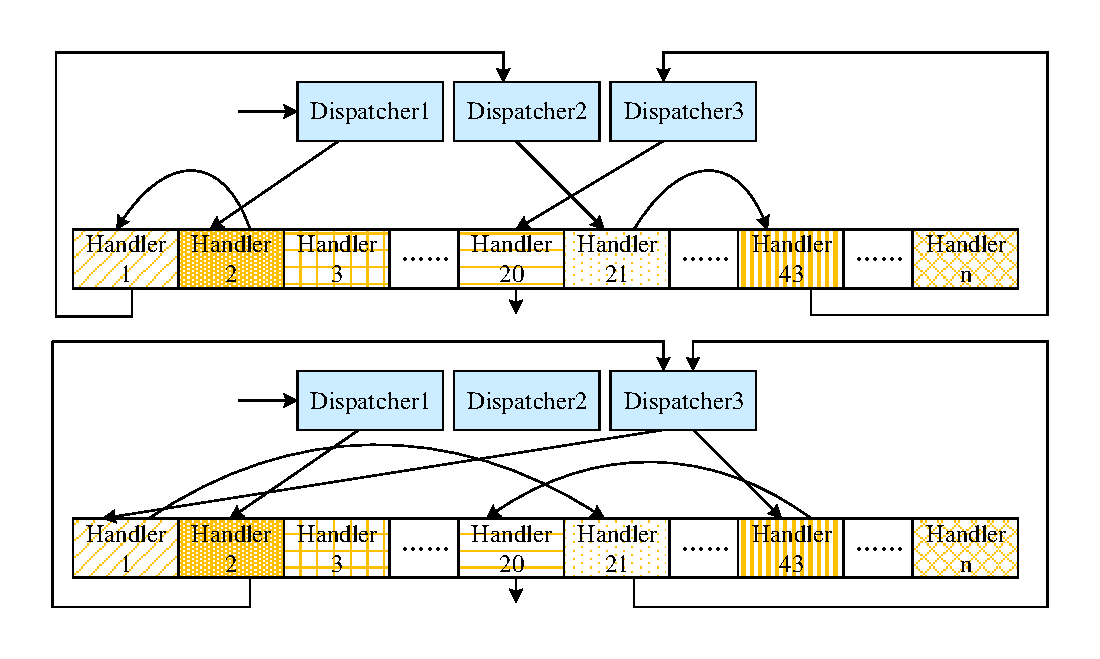
\includegraphics[width=0.9\columnwidth]{figure/figdh.pdf}\\
  \caption{Two types of possible scheduling structure. In the figure, the handlers' execution sequence is: H2$\rightarrow$H1$\rightarrow$H21$\rightarrow$H43$\rightarrow$H20. We can see that there was a big difference between the results of different runtime.}\label{fig:Fig.3}
\end{figure}
\subsubsection{Create two sets of driver-data}
Only the control unit is not enough. We also need one new set of driver-data to cooperate. As the Figure\ref{fig:Fig.2} shows, the driver-data is of great importance, which determines the handler's execution sequences. However, one set driver-data is difficult to provide random sequences and the one-to-one relationship between handler and driver-data will be clearly identified easily. To solve the above-mentioned problem, we propose two sets driver-data solution.
\par \emph{DriverData1} and \emph{DriverData2} will be introduced for describing the creating process. The \emph{DriverData1} and usual driver-data are the same and it is for dispatcher, which is composed of the handler's serial number and its parameters. The first data in \emph{DriverData2} is the handler serial number, the rest of it are composed the offset value between two adjacent handlers and parameters. If the control unit chooses to execute the next handler, it will fetch the corresponding offset value from the \emph{DriverData2}. They are all stored encrypted.
\subsubsection{Show the random structure}
The method mentioned above can simply implement the diversity of the program execution path. Once the previous handler finished, it has the option between returning dispatcher to fetch \emph{DriverData1} and accessing the \emph{DriverData2} to fetch the offset value. Obviously, if there are more dispatchers, it will have a lot more choice.
\par In order to explain how this scheduling structure works at runtime, we illustrative our results by some examples. If the key code segment needs five handlers and three dispatchers, there will be 4$^4$ sets structures to be chosen. Figure\ref{fig:Fig.3} shows two possible uncertainty structures. The execution sequences of basic block are very different, and the first attack knowledge on the control flow will be useless to the next attack directly.

\subsection{Multi-VM switch}
In the default settings, VM-based obfuscation protects the key code regions with a single VM (SVM) structure. We put forward the Multi-VM (MVM) for user to choose and which contains multiple sets of equivalent but different forms of handlers and driver-data.
\par Typically, SVM only generates one set of driver-data and handlers. No matter how complex its structure is the relationship of handler and bytecodes is fixed. This will be operable weakness for the adversary. In contrast, our MVM has a dynamic mechanism and it will provide the different handler serial numbers for different instances of protection, for the same instance, the same function handler will also have a different serial number and structure. In fact, every execution will random switch driver-data from multiple VM, and it would show different mappings between the handler and driver-data. As the adversary, if he cannot find this mapping relationship, he wouldn't restore the integrally original code and data. Next we illustrate the details of multi-VM.
\begin{figure}[t]
  \centering
  % Requires \usepackage{graphicx}
  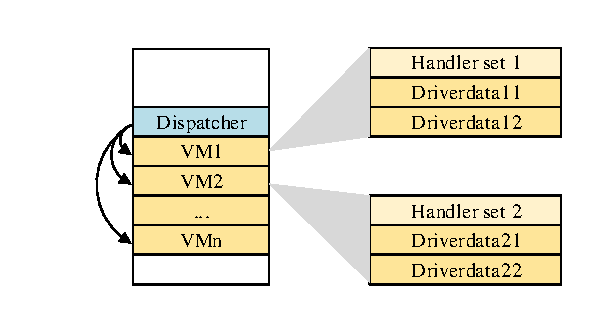
\includegraphics[width=0.8\columnwidth]{figure/figmvm.pdf}\\
  \caption{The structure of multiple VM. Each VM contains one set of unique handlers and two sets of driver-data, \emph{DriverDataSetN1} and \emph{DriverDataSetN2}.}\label{fig:Fig.4}
\end{figure}
\subsubsection{Generate multiple Handler sets}
\emph{HAS} as an original handler set that consists of \emph{n} handlers, it will be obfuscated for \emph{VMNum} times for building multi-VM, then get multiple handler sets and which are semantic equivalence but have different forms. However, all of the equivalent handlers have the same serial number. This is a kind of directly mapping relationship and is detrimental to the security of the system. So further disrupt the serial number of the handler in order to enhance the effect of obfuscation, and the relationship of these equivalent handlers in different sets should be: \emph{HAS$_1$(i)$\Leftrightarrow$HAS$_2$(j)$\Leftrightarrow$ ... $\Leftrightarrow$HAS$_{vm}$(k), }1\emph{$\leqslant$i, j, k$\leqslant$n}, it will produce variety mapping relationship of handler and VI. There are various methods to upset the handler's serial number, we take a simple method that all the serial number plus a uniform random number, then regard the result MOD \emph{m} as the new handler's serial number.
\par Given the above design, we need to consider one practical issue that is the balance of the security and performance. Depending on the design of the previous section, we need to generate two driver-data sets for each set of handler due to the variety of mapping relationship. So the more the embedded VM number is, the more secure the protected code and the bigger the file size will be.
\subsubsection{Schedulability of  Multi-VM}
\par The former dispatcher structure function only fetches the driver-data to decrypt it and dispatch handler. To schedule the multiple VM, we need to improve the dispatcher structure. The dispatcher will make choice in multiple VM at each runtime. Firstly, we calculate the driver-data offset value between the running VM and the switching VM. Then adjust the value of ESI (register), the pointer of the new driver-data address according to the offset value. All of the dispatchers and handlers will run as the same form after being improved. They all possess the random choice function. It is hard to distinguish two types structure that can enhance the concealment of dispatchers.
\par Figure \ref{fig:Fig.4} shows the multiple sets VM drive structure, every execution wills random switch driver-data from these VM, if the result is switch to VM2 from VM1, the dispatcher need to adjust value of ESI point to \emph{DriverDataSet21} of VM2 and continue to fetch driver-data to dispatch handler. On the contrary, continue to fetch the driver-data from VM1's \emph{DriverDataSet11} and continue to execute.
\section{Case Study With \DSVMP}
After discussing the designs of \DSVMP, we will give an example to illustrate how the system operates. There is a little piece of code. "00401036" and "00401038" is the instruction address. "STARTSDK" and "ENDSDK" are the Start flag and End flag of the key code segment.
\begin{verbatim}
STARTSDK
00401036 mov eax, ebx
00401038 sub eax, 03
ENDSDK
\end{verbatim}
\subsection{Process of protection}
The first, positioning and disassemble the key code segment, then we will get two x86 instructions. "mov eax, ebx" and "sub eax, 03", add two instructions, "push 40103B" and "ret", in order to jump back to execute the rest of code after exits the \DSVMP. Then convert x86 instructions to VI follow the transformation rules of design in advance, and the results as shown in Table \ref{tab:Tab.1}. Our system is stack-based, so, "load" instructions are for pushing operands into stack, and "store" instructions are for popping results out of the stack and store it into the virtual context.
\begin{table}[t]
  \centering
\begin{tabular}{|*{3}{p{2cm}|}p{1cm}|}
%{|l|l|l|l|}
  \hline
  % after \\: \hline or \cline{col1-col2} \cline{col3-col4} ...
  \textbf{Ins1} & \textbf{Ins2} & \textbf{Ins3} & \textbf{Ins4}\\
  \hline
  \hline
  \tabincell{l}{move 0x08\\load\\move 0x04\\store} & \tabincell{l}{move 0x04\\ load\\ load 0x03\\ sub\\ store\\ move 0x04\\ store}& load 0x40103b & ret \\
  \hline
\end{tabular}
  \caption{Results of the native instructions virtualization.}\label{tab:Tab.1}
\end{table}
\par We set the embedded VM as 2 (VM1 and VM2). Transforming the improved handlers using the deformation engine, generating two sets of equivalent but form different handlers, then randomly disturb the serial number and get two new sets of handlers, HAS1 and HAS2. Then, VI was encoded into bytecodes which we call the driver-data. According to HAS1, generates the \emph{DriverDataSet11}, which composed of the handler serial number and parameters, illustrated in Figure \ref{fig:Fig.5}. Then built on \emph{DriverDataSet11}, calculate the offset value and get the D\emph{riverDataSet12}. Similarly, According to VM2's HAS2 also can get two sets of driver-data \emph{DriverDataSet21} and \emph{DriverDataSet22}.
\par Then encrypt four sets of driver-data, the encryption key is kept by register EBX and it will be modified after each encryption. Here the \emph{DriverDataSet11} and \emph{DriverDataSet12} use the same key \emph{Key1}, and \emph{DriverDataSet21} and \emph{DriverDataSet22} use another key \emph{Key2}, to ensure that the encryption and decryption are symmetrical when switching the VM. Finally, fill key code segments with junk instructions, and create a new section attached to the end of the original file, which contains two sets of handlers, four sets of driver-data, ten dispatchers and other VM components, VMcontext, VMInit and VMExit, etc.
\subsection{Process of execution}
\begin{figure}[t]
  \centering
  % Requires \usepackage{graphicx}
  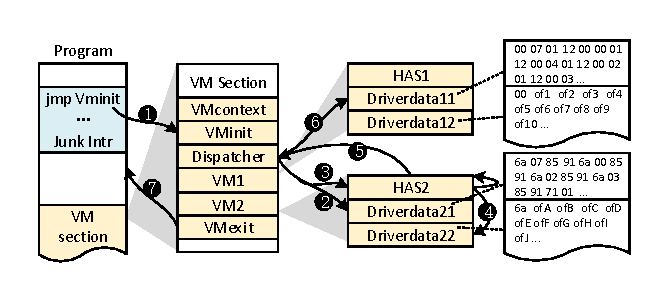
\includegraphics[width=1.0\columnwidth]{figure/figex.pdf}\\
  \caption{The execution process of protected program. Embedded VM number is 2, and each VM contains two sets of driver-data and one set of handlers.}\label{fig:Fig.5}
\end{figure}
Through the above process, software will have diversity of execution path. Specific process is shown in Figure \ref{fig:Fig.5}.
\par \textbf{Step1:} At runtime, upon executing the key code segment, a "jmp VMInit" instruction will transfer the control to the VMInit. VMInit saves the host context and initializes the virtual context, containing the initialization of the VMID, we assume it is VM2.
\par \textbf{Step2:} Next, dispatcher starts to work and it fetches a bytecode from the \emph{DriverDataSet21} decodes it gets "6a". Jump to and execute "0x6aHandler", the next bytecode "07" is its parameters.
\par \textbf{Step3:} Start executing the structure control unit when "0x6aHandler" executed over. It randomly selects to continue execution "0x85Handler" or return to the dispatcher. If choose return to the dispatcher,  move on to step 5.
\par \textbf{Step4:} The "0x6aHandler" fetches a bytecode from \emph{DriverDataSet21}, decodes it and get offset value. According to this value jumps to the "0x85Handler" continues to execution. Move on to step 3.
\par \textbf{Step5:} There are 10 dispatcher embedded. Randomly select one and jump to execute.
\par \textbf{Step6:} Execute the selected dispatcher. Select one VM randomly and complete switches VM by adjusting the pointer value of the register ESI. Fetches a bytecode from driver-data, decodes it and get the handler serial number. Then jump to the handler and back to Step3.
\par \textbf{Step7:} Step3 and Step4 are iterated until complete the all bytecodes. Then execute VMexit, which restore and jump back to native context continue to execute the left code.
\section{Security Analysis}
The protected software will show the variant execution paths in different run time, related analyses are as follows.
\subsection{Runlevel software structure similarity analysis}
In order to gather statistics on the number of all possible execution structure when the instance runs, we assume that the number of dispatcher is 10. Here, the number of the dispatcher is an optional protective option. In the case of Section VI, the length of the \emph{DriverDataSet11} and \emph{DriverDataSet21} are all 103 byte, contains a total of 78 handler serial numbers. Remove the last handler because of it will directly exit the VM when it runs over. All the rest of the 77 handlers have 11 kinds of choice. Each handler can directly jump to the next handler, or return to one of the 10 dispatcher.
\par So there is 11$^{77}$ possible execution paths. So the probability that appears the same control flow structure in a continuous operation is \[P = \frac{1}{{{{11}^{77}}}}\] Here just has one VM, if we embed 5 VM, each dispatcher also can have 5 kinds of choice. The more number of dispatcher and VM is, the more number of control flow structure will be. So we can know that the \DSVMP can make software with very low run level structure similarity.
\subsection{The code level software structure similarity analysis}
If all of the software protected by the same protection system have the exactly same features, the attacker can use these features to crack any software protected by this tool. In order to show that our system can resilient such attacks, we calculate the similarity of two software structures to assess the difficulty of attacker crack software (protected by \DSVMP).
%add new content ֤����ʽ���Ƶ�����
\par Blietz et al.\cite{18blietz2006software} present some concept to describe the structural features of control flow, like branch number, cycle index, node nesting level and so on. On the basis of existing literature, we present some indices for structural diversity, details are as follows.
\par \texttt{NodeNum}, is the number of basic blocks.
\par \texttt{BranchNum}, is the number of basic blocks which the last instruction is the conditional jump instruction.
\par $DR(Vi)$, is the basic block degree relationship of \emph{Vi}, and $DR(Vi) = {D_{in}}(Vi) + {D_{out}}(Vi)$, ${D_{out}}\left( {Vi} \right)$ refers to the out-degree and ${D_{in}}\left( {Vi} \right)$ refers to the in-degree.
\par Similarly, $DF(Vi)$ is the data flow relationship of basic block \emph{Vi}, used to indicate the frequency of \emph{Vi}'s information exchange. $DF\left( {Vi} \right){\rm{ }} = {\rm{ }}Flo{w_{in}}(Vi) + Flo{w_{out}}(Vi)$, and $Flo{w_{in}}$ is the number of reading instruction in \emph{Vi}, $Flo{w_{out}}$ is the number of writing instruction in \emph{Vi}.
\par As shown in Table \ref{tab:Tab.2}, the second column is the key code segment. Their structures are all very simple that only have one basic block and there is no branch block, the structure similarity is close to 100\%. We get A' and B' by using \DSVMP, the related information of the structure is also as shown in Table \ref{tab:Tab.2}. We use a formula to calculate the software structure information of A' and B' respectively, the results are as follows.
%��ʽ��ʽ��ʽ��ʽ��ʽ��ʽ
\[\begin{array}{l}
 SInfo{r_{A'}} = NodeNu{m_{A'}} + BranchNu{m_{A'}} \\
 {\kern 1pt} {\kern 1pt} {\kern 1pt} {\kern 1pt} {\kern 1pt} {\kern 1pt} {\kern 1pt} {\kern 1pt} {\kern 1pt} {\kern 1pt} {\kern 1pt} {\kern 1pt} {\kern 1pt} {\kern 1pt} {\kern 1pt} {\kern 1pt} {\kern 1pt} {\kern 1pt} {\kern 1pt} {\kern 1pt} {\kern 1pt} {\kern 1pt} {\kern 1pt} {\kern 1pt} {\kern 1pt} {\kern 1pt} {\kern 1pt} {\kern 1pt} {\kern 1pt} {\kern 1pt} {\kern 1pt} {\kern 1pt} {\kern 1pt} {\kern 1pt} {\kern 1pt} {\kern 1pt} {\kern 1pt} {\kern 1pt} {\kern 1pt} {\kern 1pt} {\kern 1pt} {\kern 1pt} {\kern 1pt} {\kern 1pt} {\kern 1pt} {\kern 1pt} {\kern 1pt}  + \sum\limits_{i = 0}^{i < n} {(DR(i) + DF(i))}  \\
 {\kern 1pt} {\kern 1pt} {\kern 1pt} {\kern 1pt} {\kern 1pt} {\kern 1pt} {\kern 1pt} {\kern 1pt} {\kern 1pt} {\kern 1pt} {\kern 1pt} {\kern 1pt} {\kern 1pt} {\kern 1pt} {\kern 1pt} {\kern 1pt} {\kern 1pt} {\kern 1pt} {\kern 1pt} {\kern 1pt} {\kern 1pt} {\kern 1pt} {\kern 1pt} {\kern 1pt} {\kern 1pt} {\kern 1pt} {\kern 1pt} {\kern 1pt} {\kern 1pt} {\kern 1pt} {\kern 1pt} {\kern 1pt} {\kern 1pt} {\kern 1pt} {\kern 1pt} {\kern 1pt} {\kern 1pt}  = 23 + 5 + (DR(0) + DR(1) + ... + DR(22) \\
 {\kern 1pt} {\kern 1pt} {\kern 1pt} {\kern 1pt} {\kern 1pt} {\kern 1pt} {\kern 1pt} {\kern 1pt} {\kern 1pt} {\kern 1pt} {\kern 1pt} {\kern 1pt} {\kern 1pt} {\kern 1pt} {\kern 1pt} {\kern 1pt} {\kern 1pt} {\kern 1pt} {\kern 1pt} {\kern 1pt} {\kern 1pt} {\kern 1pt} {\kern 1pt} {\kern 1pt} {\kern 1pt} {\kern 1pt} {\kern 1pt} {\kern 1pt} {\kern 1pt} {\kern 1pt} {\kern 1pt} {\kern 1pt} {\kern 1pt} {\kern 1pt} {\kern 1pt} {\kern 1pt} {\kern 1pt} {\kern 1pt} {\kern 1pt} {\kern 1pt} {\kern 1pt} {\kern 1pt} {\kern 1pt} {\kern 1pt} {\kern 1pt} {\kern 1pt} {\kern 1pt}  + DF(0) + DF(1) + ... + DF(22)) \\
 {\kern 1pt} {\kern 1pt} {\kern 1pt} {\kern 1pt} {\kern 1pt} {\kern 1pt} {\kern 1pt} {\kern 1pt} {\kern 1pt} {\kern 1pt} {\kern 1pt} {\kern 1pt} {\kern 1pt} {\kern 1pt} {\kern 1pt} {\kern 1pt} {\kern 1pt} {\kern 1pt} {\kern 1pt} {\kern 1pt} {\kern 1pt} {\kern 1pt} {\kern 1pt} {\kern 1pt} {\kern 1pt} {\kern 1pt} {\kern 1pt} {\kern 1pt} {\kern 1pt} {\kern 1pt} {\kern 1pt} {\kern 1pt} {\kern 1pt} {\kern 1pt} {\kern 1pt} {\kern 1pt} {\kern 1pt}  = 28 + (46 + 18){\kern 1pt} {\kern 1pt} {\kern 1pt} {\kern 1pt} {\kern 1pt} {\kern 1pt}  = {\kern 1pt} {\kern 1pt} {\kern 1pt} {\kern 1pt} 92 \\
 \end{array}\]
\[\begin{array}{l}
 SInfo{r_{B'}} = NodeNu{m_{B'}} + BranchNu{m_{B'}} \\
 {\kern 1pt} {\kern 1pt} {\kern 1pt} {\kern 1pt} {\kern 1pt} {\kern 1pt} {\kern 1pt} {\kern 1pt} {\kern 1pt} {\kern 1pt} {\kern 1pt} {\kern 1pt} {\kern 1pt} {\kern 1pt} {\kern 1pt} {\kern 1pt} {\kern 1pt} {\kern 1pt} {\kern 1pt} {\kern 1pt} {\kern 1pt} {\kern 1pt} {\kern 1pt} {\kern 1pt} {\kern 1pt} {\kern 1pt} {\kern 1pt} {\kern 1pt} {\kern 1pt} {\kern 1pt} {\kern 1pt} {\kern 1pt} {\kern 1pt} {\kern 1pt} {\kern 1pt} {\kern 1pt} {\kern 1pt} {\kern 1pt} {\kern 1pt} {\kern 1pt} {\kern 1pt} {\kern 1pt} {\kern 1pt} {\kern 1pt} {\kern 1pt} {\kern 1pt} {\kern 1pt}  + \sum\limits_{i = 0}^{i < m} {(DR(i) + DF(i))}  \\
 {\kern 1pt} {\kern 1pt} {\kern 1pt} {\kern 1pt} {\kern 1pt} {\kern 1pt} {\kern 1pt} {\kern 1pt} {\kern 1pt} {\kern 1pt} {\kern 1pt} {\kern 1pt} {\kern 1pt} {\kern 1pt} {\kern 1pt} {\kern 1pt} {\kern 1pt} {\kern 1pt} {\kern 1pt} {\kern 1pt} {\kern 1pt} {\kern 1pt} {\kern 1pt} {\kern 1pt} {\kern 1pt} {\kern 1pt} {\kern 1pt} {\kern 1pt} {\kern 1pt} {\kern 1pt} {\kern 1pt} {\kern 1pt} {\kern 1pt} {\kern 1pt} {\kern 1pt} {\kern 1pt} {\kern 1pt} {\kern 1pt}  = 48 + 9 + (DR(0) + DR(1) + ... + DR(47) \\
 {\kern 1pt} {\kern 1pt} {\kern 1pt} {\kern 1pt} {\kern 1pt} {\kern 1pt} {\kern 1pt} {\kern 1pt} {\kern 1pt} {\kern 1pt} {\kern 1pt} {\kern 1pt} {\kern 1pt} {\kern 1pt} {\kern 1pt} {\kern 1pt} {\kern 1pt} {\kern 1pt} {\kern 1pt} {\kern 1pt} {\kern 1pt} {\kern 1pt} {\kern 1pt} {\kern 1pt} {\kern 1pt} {\kern 1pt} {\kern 1pt} {\kern 1pt} {\kern 1pt} {\kern 1pt} {\kern 1pt} {\kern 1pt} {\kern 1pt} {\kern 1pt} {\kern 1pt} {\kern 1pt} {\kern 1pt} {\kern 1pt} {\kern 1pt} {\kern 1pt} {\kern 1pt} {\kern 1pt} {\kern 1pt} {\kern 1pt} {\kern 1pt} {\kern 1pt}  + DF(0) + DF(1) + ... + DF(47)) \\
 {\kern 1pt} {\kern 1pt} {\kern 1pt} {\kern 1pt} {\kern 1pt} {\kern 1pt} {\kern 1pt} {\kern 1pt} {\kern 1pt} {\kern 1pt} {\kern 1pt} {\kern 1pt} {\kern 1pt} {\kern 1pt} {\kern 1pt} {\kern 1pt} {\kern 1pt} {\kern 1pt} {\kern 1pt} {\kern 1pt} {\kern 1pt} {\kern 1pt} {\kern 1pt} {\kern 1pt} {\kern 1pt} {\kern 1pt} {\kern 1pt} {\kern 1pt} {\kern 1pt} {\kern 1pt} {\kern 1pt} {\kern 1pt} {\kern 1pt} {\kern 1pt} {\kern 1pt} {\kern 1pt} {\kern 1pt} {\kern 1pt}  = 57 + (96 + 36){\kern 1pt} {\kern 1pt} {\kern 1pt} {\kern 1pt}  = {\kern 1pt} {\kern 1pt} {\kern 1pt} {\kern 1pt} {\kern 1pt} 189 \\
 \end{array}\]
\begin{table}
  \centering
  \begin{tabular}{|c|c|c|c|c|c|c|}
%{|p{0.95cm}|p{1.4cm}|p{0.55cm}|p{0.55cm}|p{0.95cm}|p{0.55cm}|p{0.55cm}|}
     \hline
    \multicolumn{4}{|c|}{\textbf{Basic info of target program}}& \multicolumn{3}{|c|}{\textbf{Info of protected-software}} \\
     \hline
     \hline
     % after \\: \hline or \cline{col1-col2} \cline{col3-col4} ...information of protected software
     \textbf{prog.} & \textbf{key code} & \textbf{\tabincell{l}{Dis\\Num}} & \textbf{\tabincell{l}{VM\\Num}} & \textbf{prog.} & \textbf{\tabincell{l}{Node\\Num}} & \textbf{\tabincell{l}{Branch\\Num}}\\
     \hline
     \hline
     A & \tabincell{l}{mov eax,ebx\\sub eax,03} & 5 & 5 & A' & 23 & 5\\
     \hline
     B & \tabincell{l}{pop eax\\add eax,ebx} & 10 & 10 & B' & 48 & 9 \\
     \hline
   \end{tabular}
  \caption{The relevant information about the program.}\label{tab:Tab.2}
\end{table}
\par From the $SInfo{r_{A'}}$ and $SInfo{r_{B'}}$, we can calculate the software structure similarity $SDiff$ of A' and B'.
%��ʽ
\[SDiff = \frac{{|SInfo{r_{A'}} - SInfo{r_{B'}}|}}{{SInfo{r_{A'}} + SInfo{r_{B'}}}}\;{\kern 1pt}  = \frac{{97}}{{281}} = 34.5\% \]

\par Thus it can be seen the software structure similarity between A' and B' is only 34.5\%, \DSVMP has greatly increased the difficulty that the attacker perform the dynamic attack by using control flow and data flow information.

\section{Performance Evaluation}
In this section, we present a detailed discussion about experiment and cost analysis, and then evaluate the effectiveness of \DSVMP based on the experimental data in detail.
\subsection{Security experimental evaluation}
We verify the security of \DSVMP by using an attack experiment, and the number of VM and dispatcher in the instance is set at 3 and 5.
\par Using the tool "IDA"\cite{14Idapro} to debug the instances,and then locate the start tag of key code segment and get the control flow graph of the program after into the virtual machine, but the last one basic block ended in an indirect jump instruction, "IDA" can not automatic acquisition the target address, so it is incomplete. We need to collect the dynamic instructions, and then manually connect the basic block to draw a complete control flow graph. By utilizing taint analysis and control dependencies to simplify and extract the software structure information. But the control flow structure has changed when we try to analyze the software again, previous attack experience is useless, we can only take time again to draw complete control flow graph in current state.
\par Then we use a tool "OllyDbg"\cite{15Ollydbg} to perform the dynamic debugging, and then locate the dispatcher. Register ESI points to the driver-data, defining the ESI for tainted data and track its transmission process, we can find that the dispatcher fetchs the bytecode and stores it in register EAX after decryption, these are the serial number of the handler. Collect all values that scheduled by each dispatcher, as follows:
%\begin{verbatim}
%00 0A 12 15 37 64 00 0A 12 89 0B 02 57 36
%78 9A 8E 65 0C 13 25 32 11 24 0A 12 24 8F
%4E 35 34 01 02 07 12 24 09 2A 31 44 05 01
%0F 12 34 52 35 09 01 65 81 33 01 0A 07 12
%34 25 36 93 78 32 57 04 05 01 30 4C 3D 67
%13 45 21 01 03 07
%\end{verbatim}
\begin{verbatim}
00 0A 12 15 37 64 00 0A 12 89 0B 02 57 36
78 9A 8E 65 0C 13 25 32 11 24 0A 12 24 8F
4E 35 34 01 02 07 12 24 09 2A 31 44 05 01
0F 12 34 52 35 09 ... ...
\end{verbatim}
\par But these serial numbers are composed of multiple VM, and it is incomplete because some handlers did not schedule through the dispatcher. So it is difficult to distinguish the relationship between these handler serial numbers and VMID. \DSVMP embed multiple sets of handler in virtual interpreter, the attacker wants to analyze these handler completely is very difficult. Even it can be fully analyzed, we still unable to crack the software, because we don't know the relationship of handler serial number and set of handler.

\subsection{Runtime cost evaluation}
We evaluate the performance impact of \DSVMP on a PC with Intel$^{\circledR}$ Core$^{TM}$ 2 Duo processor at 3.00GHz with 4.00GB of RAM. The operating system environment is Windows 7. We selected four test cases. They respectively are md5.exe\cite{19md5}, aescrypt.exe\cite{20Aescrypt}, bcrypt.exe\cite{21bcrypt}, and gzip.exe\cite{22gzip}, they are all used to process a file (test.jpg) of the size 763KB. Table III shows the basic information of these target programs. The 3th column indicates the critical function and the 4th column indicates the number of instructions in these critical functions. The numbers of instructions executed in the critical functions while processing the ��test.jpg�� file is shown in the last column.
\subsubsection{Impact on File Size and Runtime Performance}
For each target program, we use the prototype of \DSVMP to protect it for 5 times, each time using a different number of VM. Figure \ref{fig:Fig.6} (a) shows the impact on file size of \DSVMP with multi-VM protection. Since each VM has two sets of driver-data and one set of handlers, the file size of the protected program increases as the number of VM increases. Besides, exist a positive correlation between the sizes of and the number of critical instructions, so "aescrypt" has the fastest increasing of file size, "bcrypt" is slowest.
\par To evaluate the runtime overhead that \DSVMP introduces, we use each programs to process the "test.jpg" file for 10 times. Then we calculate the average runtime overhead per critical instruction and the results are shown in Figure \ref{fig:Fig.6} (b). The runtime overhead increases as the number of VM increases. But 3VM always has a lower overhead than 2VM, this is not just a coincidence, one possible reason is the implementation strategy we use in multi-VM protection. Besides, "aescrypt" has a much higher runtime overhead that other program. Because its critical code more complex and needs more virtual instructions to interpret.

\subsubsection{Comparison with two commercial VM-based protection tools}
To illustrate the applicability of \DSVMP, we compare it with two commercial VM protection systems, Code Virtualizer~\cite{2CV} and VMProtect~\cite{3Vmprotect}. As we only compare the impact of code virtualization protection, we disable other protection techniques that integrated into VMProtect and CV, e.g., code compression, resource protection, etc. Besides, CV has 24 custom VMs that are devised ahead of protection, and we choose one of moderate complexity and speed, namely the FISH32 (White), to protect. As for \DSVMP, it with 2 VMs. Figure \ref{fig:Fig.7} (a) shows the impact on file size of three different VM protection systems. CV has the fastest increasing of file size, but the increasing of the size is relatively stable and independent on original program size; this is true for \DSVMP and VMProtect as well. Figure \ref{fig:Fig.7} (b) introduces the comparison of three VM protection systems on average runtime overhead. CV has the largest runtime overhead while VMProtect the smallest and \DSVMP the moderate.
\par \DSVMP improved the atom handler, operations of the control unit will cost some time overhead, and embedded the multiple VM also will increase the volume. In general, our approach gets a better performance.
\begin{table}
  \centering
  \begin{tabular}{|c|c|c|c|c|}
     \hline
     % after \\: \hline or \cline{col1-col2} \cline{col3-col4} ...information of protected software
     \textbf{prog.} & \textbf{Size(KB)} & \textbf{Critical code} & \textbf{\tabincell{l}{Instr.\\Protect}} & \textbf{\tabincell{l}{Instr.\\Executed}}\\
     \hline
     \hline
     md5 & 11 & Transform() & 563 & 6869163\\
     \hline
     aescrypt & 142 & encrypt-stream() & 1045 & 5502747\\
     \hline
     bcrypt & 68 & Blowfish-Encrypt() & 54 & 43945017\\
     \hline
     gzip & 56 & deflate() & 154 & 35877278\\
     \hline
   \end{tabular}
  \caption{The basic information of the target program.}\label{tab:Tab.3}
\end{table}
\begin{figure}[t]
\centering
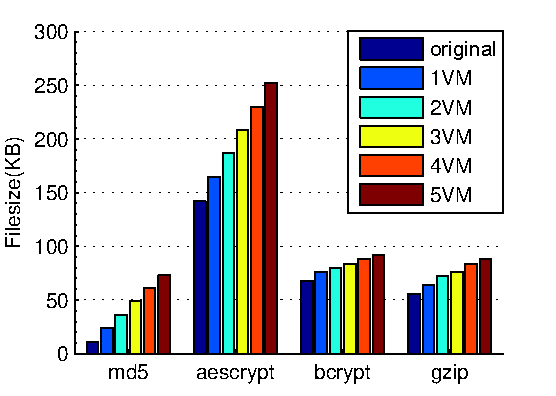
\includegraphics[width=.24\textwidth]{figure/fig6a.pdf}
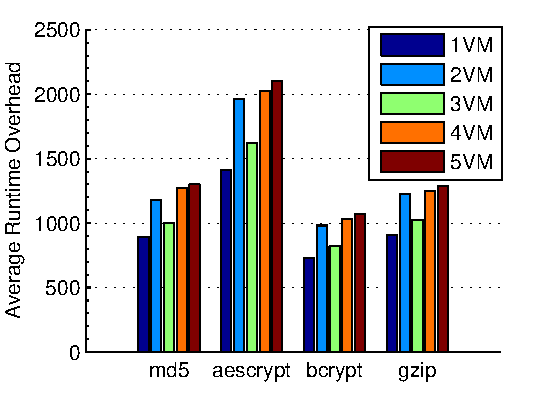
\includegraphics[width=.24\textwidth]{figure/fig6b.pdf}
\caption{(a) The impact on file size (KB) of \DSVMP that embedded different VM. (b) The average runtime overhead per critical instruction use the different number of VM protection.}\label{fig:Fig.6}
\centering
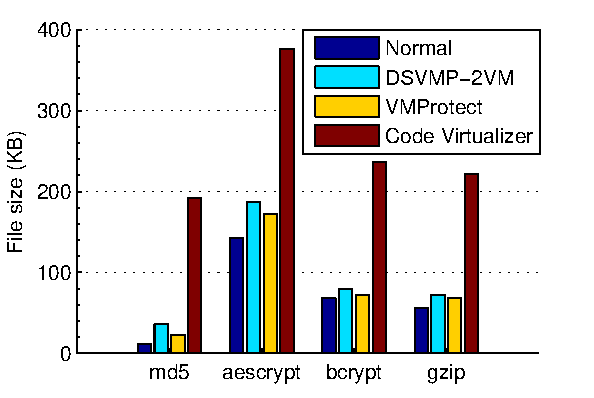
\includegraphics[width=.24\textwidth]{figure/fig7a.pdf}
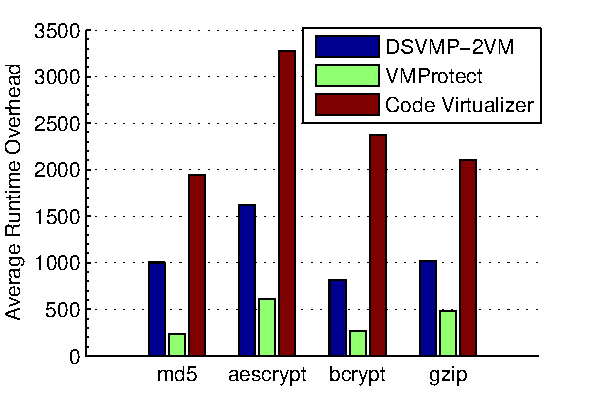
\includegraphics[width=.24\textwidth]{figure/fig7b.pdf}
\caption{(a) The comparison of impact on file size (KB) with VMProtect and Code Virtualizer. (b) The comparison of average runtime overhead per dynamically executed critical instruction with VMProtect and Code Virtualizer.}\label{fig:Fig.7}
\end{figure}
\section{Related Work}
Early works on the binary code protection relied on some simple encryption and obfuscation methods, however, these approaches can only provide limited protection when faced with complex diversified attacks. Typically, junk instructions\cite{23linn2003obfuscation}, packers\cite{25Execryptor,26upx}, above technology usually are used to resist disassembly and some static analysis. There are code obfuscation\cite{25wu2010mimimorphism}, control flow and data flow obfuscation\cite{13liem2008compiler,27ge2005control,27balachandran2014function}, etc. which are mainly used to obfuscate the semantic and logical information of the target program. So in practical applications, these approaches are seldom caught alone, and they usually combine with each other to protect an instance.
\par There is a growing interest in using code virtualization to protect the software from malicious reverse engineering. We've already introduced the general process of classical VM-based protection in section II and some possible attacks in section III. Here are some of the research work focuses on VM-based protection. Fang et al.\cite{5fang2011multi} proposed a protection scheme that is a multi-stage obfuscation, which transforms the critical code iteratively for many times by using different interpretations to improve security. Yang et al.\cite{6ming2011software} presents a nested virtual machine, and the adversary has to reverse engineer fully each layer of the interpreter step by step before to the next layer. Averbuch et al.\cite{27averbuch2011efficient} introduces the encryption and decryption technology on the basis of VM-based protection, which uses the AES algorithm and the custom encryption key to encrypt the virtual instructions, at runtime, the first decrypt the virtual instruction and then dispatch a handler to interpret it. Wang et al.\cite{7wang2014tdvmp} put forward the time diversity, which constructs several equivalent but different forms sub paths, and these sub paths will be randomly selected to achieve the diversity at runtime.
\par \DSVMP presents the dynamic instruction scheduling structure to improve security for software: (i) Improving the atom handler, add a structure control unit for it to realize the diversified scheduling. (ii) Embedded multiple VM, at runtime, the VM interpreter will fetch the execution data from multiple sets of driver-data randomly and to further obfuscate the semantics of bytecode instructions. Software diversity is an effective strategy to prevent mass scale exploitation and cracking\cite{20larsen2014sok}. Our system by applying the above approach to provide internal diversity further impedes the reverse attack.


\section{Conclusion}
In this paper, we introduce the details of improved VM-based protection called \DSVMP, it proposes improved diversity scheduling structure and multiple VM to mitigate the vulnerability of the classical VM. We show the implementation process of our system, and we also analyze and evaluate that our \DSVMP is practical and effective for resilient the dynamic accumulation attacks.
\par \DSVMP also has vulnerability, multi-VM randomly selected by the dispatcher's selection structure, and in MVM, each VM can independently finish the complete function. Although the handler also has a random select structure that improves the concealment of dispatcher, once the adversary locates the dispatcher, they can tamper with the control structure to affect the results of selection, so that MVM will be failure.
\par We intend to increase the tamper-proof technology into our system. Further, we can add a security thread library, contains of the anti-debug and anti-dump threads etc. We also can improve the virtual instruction set and driver-data to make each VM only contains part of the whole driver-data, so that the adversary has to analyze the different VMs.
% conference papers do not normally have an appendix

% use section* for acknowledgment
\section*{Acknowledgment}
This work was partial supported by project National Natural Science Foundation of China (No. 61373177, and No. 61572402), the Key Project of Chinese Ministry of Education (No. 211181), the International Cooperation Foundation of Shaanxi Province, China (No. 2013KW01-02, No. 2015KW-003 and No. 2016KW-034), the China Postdoctoral Science Foundation (grant No. 2012M521797), the Research Project of Shaanxi Province Department of Education (No. 15JK1734), the Research Project of NWU, China (No. 14NW28), and the UK Engineering and Physical Sciences Research Council under grants EP/M01567X/1 (SANDeRs), EP/M015793/1 (DIVIDEND).

%The authors would like to thank...

% trigger a \newpage just before the given reference
% number - used to balance the columns on the last page
% adjust value as needed - may need to be readjusted if
% the document is modified later
%\IEEEtriggeratref{8}
% The "triggered" command can be changed if desired:
%\IEEEtriggercmd{\enlargethispage{-5in}}

% references section

% can use a bibliography generated by BibTeX as a .bbl file
% BibTeX documentation can be easily obtained at:
% http://mirror.ctan.org/biblio/bibtex/contrib/doc/
% The IEEEtran BibTeX style support page is at:
% http://www.michaelshell.org/tex/ieeetran/bibtex/
%\bibliographystyle{IEEEtran}
% argument is your BibTeX string definitions and bibliography database(s)
%\bibliography{IEEEabrv,../bib/paper}
%
% <OR> manually copy in the resultant .bbl file
% set second argument of \begin to the number of references
% (used to reserve space for the reference number labels box)

%\begin{thebibliography}
%\bibitem{IEEEhowto:kopka}
%H.~Kopka and P.~W. Daly, \emph{A Guide to \LaTeX}, 3rd~ed.\hskip 1em plus
%  0.5em minus 0.4em\relax Harlow, England: Addison-Wesley, 1999.

\bibliographystyle{IEEEtran}
\bibliography{reference}

%\end{thebibliography}14Ida pro14Ida pro14Ida pro14Ida pro
% that's all folks
\end{document}


